\chapter[Livelihoods and food security in an urban linked, high potential region of Tanzania: Changes over a three-year period]{Livelihoods and food security in an urban linked, high potential region of Tanzania: Changes over a three-year period}
\chaptermark{Livelihoods and food security in an urban linked, high potential region of Tanzania}
\label{cha:chapter4}
\vspace*{\fill}
This chapter is based on:
\\
\\
% Full citation of the published (or submitted/in review) article
% This refers to the article key in the refs.bib file.

%\bibentry{Fraval2018a}


Fraval, S., Hammond, J., Lannerstad, M., Oosting, S. J., Sayula, G., Teufel, N., Silvestri, S., Poole, E. J., Herrero, M., van Wijk, M. T. (2018). Livelihoods and food security in an urban linked, high potential region of Tanzania: Changes over a three year period. \textit{Agricultural Systems, 160 (January 2018)}, 87–95. doi:10.1016/j.agsy.2017.10.013



\newpage

\section*{Abstract}
Projected changes to rural communities in sub-Saharan Africa (SSA) are unprecedented in scale and pace. This paper investigates to what extent significant changes in livelihoods, poverty and food security performance are already taking place. The study focuses on households in Lushoto district (n = 147), a remote but urban linked area of Tanzania. Within the short time period between 2012 and 2015, 77\% of households made changes in farm resources or farm characteristics. Households in the study site can be broadly classified as `Rising high value crop', `Rising livestock', `Subsisting mixed' and `Subsisting crops'. Some of the most substantial changes we observed in the three year period of study were most likely not related to any of the agricultural orientated interventions that are being promoted in the region, but are likely endogenous changes. The land expansion seen in the `Rising' households (n = 58) provides a counterpoint to the trend established in the literature of decreasing farm sizes across lower income countries more broadly, and specifically in Africa. The strategy of land expansion is risky, potentially representing a future of winners and losers, ultimately with some landholders falling further into poverty rather than leveraging their agricultural enterprises to improve their well-being. Our results show that in sites like Lushoto with a good rural to urban connection (increasingly common in SSA), households can be agile and diverse. This means that agency interventions are aiming for a moving target. In order to achieve income and food security outcomes, targeted and rapid monitoring tools will be needed.

\newpage

\section{Introduction}

The projected changes to rural communities in sub-Saharan Africa (SSA) are unprecedented in scale and pace. Global population projections in 2050 exceed 9.5 billion people, with the greatest growth to be seen in SSA nations -- increasing to 22\% of the global population (from 13\% in 2015; \citealp{UnitedNations2015}). The average rate of rural to urban migration in SSA between 1990 and 2000 was low, at 1.07\% (\citealp{deBrauw201433}); this rate of migration is forecast to remain low, contributing to a net increase in the rural SSA population from 579 million in 2014 to 938 million in 2050 (\citealp{UnitedNations2014}). In this context, the dynamics within rural communities will undoubtedly change, influencing livelihoods, human nutrition and the environmental base on which these depend. While the full effect of these changes may be some years away, there is evidence that rural communities are already undergoing rapid transformation.

Tanzania is one example of an African country showing rapid economic progress. Since the reformation of the East African Community in 1999, the Tanzanian economy has performed well (GDP in 2015 was 6 times that of 2000), growing consistently by 7\% from 2013 to 2015 (\citealp{NationalBureauofStatisticsTanzaniaNBS2016}). Agriculture has remained a significant contributor to Gross Domestic Product (GDP; {\textgreater}28\%) and is the sector employing the majority of the population (70\%; \citealp{NationalBureauofStatisticsTanzaniaNBS2015}; \citealp{IFAD2016}). Despite this strong economic growth, rural poverty and food insecurity are still high, with between 7.7 and 7.9\% of households experiencing both poverty and food insecurity in 2010/11 and 2012/13 respectively (\citealp{NationalBureauofStatisticsTanzaniaNBS2014}).

The future of food security in rural and urban communities in Tanzania will be influenced by population dynamics as well as changing livelihood opportunities and threats. The population in Tanzania is forecast to increase from 55 million in 2014 to 129 million in 2050. Although urban dwellers will be in the majority (53\% of the population), the rural population will have increased 1.7 times in absolute terms (United Nations, 2014). These estimates indicate that there will be drastic transformations for the rural population in terms of a rising urban majority requiring more food and increased local pressure from a growing rural population. These trends will necessitate improvements in agricultural productivity and more employment opportunities in both rural and urban areas (\citealp{IFAD2016}; \citealp{Jayne2014}).

To-date, relatively few studies have assessed the relationship between changing rural livelihoods and food security. Rather, the vast majority of related studies either a) assess the relationship between rural household characteristics and food security (often limited to diet diversity) for one year (e.g. \citealp{Bellon2016}; \citealp{Koppmair2017325}; \citealp{Luckett20152479}; \citealp{MKaibi2015}; \citealp{Sibhatu201510657}; \citealp{Snapp2015}; and, \citealp{Dillon2014}), or b) assess rural household characteristics over time without incorporating metrics on food security (e.g. \citealp{Ollenburger2016}; \citealp{Valbuena20151395}; \citealp{Ulrich2012241}; \citealp{Orr20011325}). Further, studies that have observed rural households over time and incorporated an aspect of food security either have limitations in scope or representativeness. \citet{Jones2016}, for example, investigates changes in diet diversity over time (2010 to 2013) for a large number of households in Malawi (n = 3000); this study, however, focuses on the relationship with crop species richness rather than the broader context of changing livelihoods. \citet{Falconnier2015} investigates farm trajectories (over 17 years), with a limited number of farms (n = 32) and only incorporates food self-sufficiency as a metric of food security.

This study observes households from 20 villages in Lushoto district, Tanzania, over a short timespan (3 years). The site's rapid economic growth (Regional GDP increasing by 78\% between 2012 and 2015; \citealp{NationalBureauofStatisticsTanzaniaNBS2016}), favourable agro-climatic conditions and improving rural-urban infrastructure (i.e. improved roads, electrification and telecommunications) makes it conducive to 1) realising the poverty and hunger oriented Sustainable Development Goals (\citealp{Frelat2016458}; \citealp{Dorward2009}; \citealp{Pender2001}); and 2) observing a variety of livelihood based responses to opportunities (farm and non-farm business opportunities from a growing economy and population and improved technologies) and threats (e.g. climatic or market-based). In doing so we investigate the extent to which significant changes in livelihoods, poverty and food security performance are already taking place. Of particular interest is how these insights can help in designing interventions to raise the standard of living for differing groups within communities.

\section{Methods}

\subsection{Study area}

This study is focused on households in the western Usambara highlands, Lushoto district, Tanzania (shown in Figure \ref{map:04_1}). Twenty villages were sampled from seven contiguous wards, chosen to represent the wide range of surrounding agro-ecosystems (\citealp{Rufino2013}). The site ranges in elevation from 780 to 2010 m above sea level. Rainfall is bi-modal, ranging from 690 to 1230 mm per annum, with heavier rains occurring from March to May, and from October to December. Soil types vary along the topographic gradient, progressing from limited and shallow soils (Regosols and Lithic Leptosols) on the peaks, to more developed soils (Cutanic Acrisols and Ferralic Cambisols) and then to alluvial and wet soils in the valleys (Mollic Gleyic Fluvisols and Fluvic Gleysols; Massawe 2011). Many cultivated soils are degraded, with low levels of soil organic carbon indicating limited nutrient retention capacity (\citealp{Winowiecki2016263}), and observed deficiencies in phosphorus and nitrogen (\citealp{Ndakidemi2006}). This site is an important catchment for the Pangani basin and hosts rich biodiversity sheltered by ancient forests.

\begin{figure}
  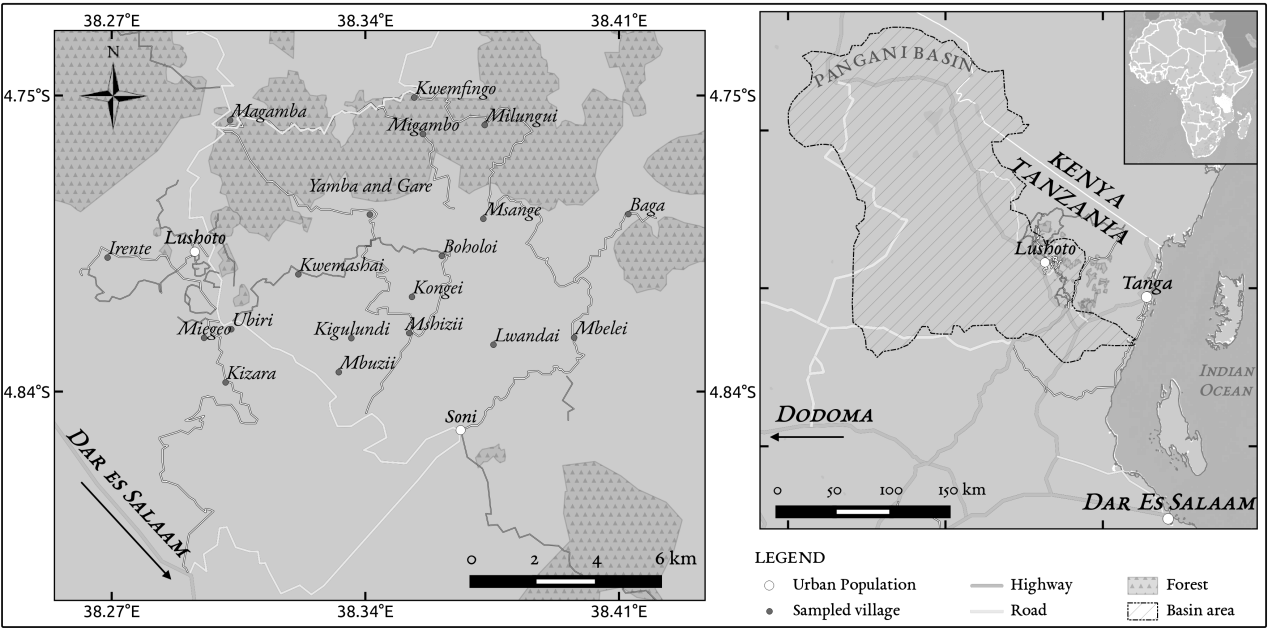
\includegraphics[width=0.9\textwidth]{figs_04/image1.png}
  \captionsetup{singlelinecheck = false, justification=justified} %left justify caption
  \caption{Study area, market infrastructure and environmental interactions}
  \label{map:04_1}
  %\small
  %\raggedright
  \vspace*{-3mm}
  \caption*{(Authors' composition based on GADM database and Open Street Maps)}
\end{figure}




The Usambara massif is densely populated by three ethnic communities: The Shambaa, Pare and Mbugu peoples (\citealp{Lyamchai2011}). Tribal social networks are still important but have become less distinctive in contemporary society, often secondary to family and religious networks (Islam and Christianity). A unique element of the culture and history in the Usambara highlands related to food security and soil conservation is that ``Access to unimproved subsistence land ... was still accepted as every resident's right... right up until the end of 1988'' (\citealp{Feierman1990}, p. 183). Modern livelihoods are largely based on agriculture and micro-enterprises, with some garnering formal employment, and others migrating to urban centres. In the villages of interest to this study, households generally have small land-holdings with a high dependency on agriculture (\citealp{Lyamchai2011}).

Several development activities have focused their efforts on the Usambara highlands, including projects on dairy, potatoes, sweet potatoes, forestry and bee-keeping. Three agricultural interventions were implemented at the time of this study (excluding forestry). One project released new bean varieties suited to the region (\citealp{Kimeli2014}); the second project trialled new potato varieties and provided farmer training on cultivation and value-chains in one of the study site's villages (namely Boheloi; \citealp{Harahagazwe2016}; \citealp{Harahagazwe2014}); the third project on dairy development, established trial plots of cultivated fodder, facilitated village level planning and worked to improve value-chain linkages. This dairy oriented project was implemented in four villages in the study site (namely Mbuzii, Ubiri, Kwemashai, Lwandai; \citealp{Kilelu20171102}). Government initiatives at multiple levels have also been working towards extending and improving the standard of the road network, electrification grid, water supply system, medical facilities and schools.

\subsection{Data collection}

Households in the study area were originally interviewed in July 2012. Data collection in 2012 was part of the Africa and South-East Asia wide CCAFS project, IMPACTlite. In Lushoto district, 200 households were sampled for IMPACTlite, being 10 households per village in a multi-stage clustered sampling design. Households were sampled based on a random geographic distribution of points within village boundaries -- as detailed in \citet{Rufino2013}. The survey was designed to collect details on farm inputs/outputs, farm activities, labour allocation, asset ownership, income and food security over a one year period. The survey's purpose was to be able to represent within site variability of livelihood indicators and provide insights into key performance indicators in terms of farm performance, food security, and the environment (\citealp{Rufino2013}).

In June-July 2015 a total of 147 households were re-sampled, with random selection at the village level resulting in six to eight households per village. Not all 200 households from 2012 were re-sampled; sampling in 2012 was more conservative as there was more uncertainty about variation between households in the site. The Rural Household Multi-Indicator Survey (RHOMIS) was utilised to represent livelihood strategies and some temporally consistent performance indicators (namely: food availability and household diet diversity). The RHOMIS tool evolved out of the IMPACTlite tool and has been designed to collect reliable information at minimum burden on respondents, providing a rapid characterisation of farm systems and performance indicators (\citealp{Hammond2017225}). This revised tool was used instead of the original IMPACTlite survey, as it collected information relevant only to a clear set of research questions and thus kept the burden to the farmer at a minimum. Interviews were conducted in Swahili and local tribal dialects by three trained enumerators and to a lesser extent by the first author. Enumerators differed from 2012, but the original site coordinator was closely engaged and worked with the enumerators in the study site to improve consistency and reduce biases that could be introduced by the way questions were phrased.

Village leaders and extension officers were interviewed concurrently to the household level interviews; in total 16 village level interviews were conducted. Topics of discussion included: changes in population, changes in land size, the importance of particular crops/livestock, livestock productivity, the condition of infrastructure and development activities (local, government or NGO led).

Additionally, insights were drawn from publicly available remote sensing products, namely: the `global satellite rain gauge', vegetative index and estimated soil properties.

\subsection{Analysis}

Using the paired observations over 2012 and 2015, this study analyses the financial and food security performance of differing adaptive responses for 147 households (thus excluding 53 out of the 200 households sampled in 2012). Changes between 2012 and 2015 were first assessed at the aggregate level. Summaries of the central tendency and distribution of households were provided for variables related to resource endowments (e.g. land, livestock and off-farm income), farm characteristics and performance indicators. As several variables of interest were not normally distributed, the central tendency was represented by the median and the distribution as the inter-quartile range (IQR).

Following on from analysis at the aggregate level, a hierarchical K-means clustering algorithm (\citealp{Kassambara2016}) then incorporated variables that would differentiate households in terms of long-term (strategic) and short-term (tactical) configurations of resources and farm characteristics -- termed `adaptive responses'. Variables included were: household population (in adult equivalents), total land cultivated, crop market participation (percentage of crop production sold), crop diversity (number of different crops grown), importance of high value crops (percentage of the area grown), crop-livestock integration (manure and crop residue utilisation), livestock-holdings and livestock market participation (percentage of livestock products sold) and off-farm income. Off-farm income was collected differently in 2012 and 2015. To maintain consistency, only income from business and employment was included, which was then evaluated as a percentage of total income. Market participation was assessed on a kilo-calorie basis (\% sold), providing a common unit of comparison across crops and livestock products. The final inputs into the clustering algorithm included the variables listed above from 2015 as well as the difference between 2015 and 2012 for each variable, all of which were centred and scaled.

Food security and poverty indicators were calculated using standardised methodologies as described in \citet{Hammond2017225}. The `household diet diversity score' (HDDS) is based on a count of a total of 12 food groups consumed (\citealp{Swindale2006}) with recall of `flush' and `lean' periods. The `household food insecurity access scale' (HFIAS) is based on nine questions on the household's experience of food insecurity for the flush and lean periods; touching on sensitive issues for the respondents such as missed meals and consumption of undesirable foods (\citealp{Coates2007}). The progress out of poverty index (PPI) is based on a country-specific set of 10 questions, scoring households from 0 to 100 (with higher scores increasingly less likely to be below the poverty line; Grameen, n.d.). Food availability is a supply and purchase potential estimate based on production, off-farm income and cost of a key staple food (maize; \textit{Zea mays L.}), expressed as Potential Food Equivalent (PFE) energy (kilocalories) per adult equivalent per day; a common calorie content was taken over the time period, with varying staple food price. It should be noted that the purchase potential from farm income has limitations as it is based on revenue rather than profit. Thus, food availability is calculated as follows (Eq. 4.1) and further detailed in \citet{Frelat2016458}.

\begin{equation}
\tag{4.1}
PFE = \frac{E_{cons} + E_{income}}{365 \times n_{hh}}
\end{equation}
%PFE = \textbackslash frac\{E\_\{cons\} + E\_\{income\}\}\{365 \textbackslash times n\_\{hh\}\} \textbf{(1)}

Remotely sensed products were used as explanatory variables for differences between years and clusters. Estimated monthly rainfall for the study site was used to identify variations from long-term average rainfall across the site as a whole (\citealp{Janowiak1999}). Additionally, the enhanced vegetative index (EVI; NASA, n.d.), soil organic carbon (SOC) and pH estimates were extracted for the households where reliable GPS coordinates were collected (n=78 due to GPS errors; estimation of soil properties detailed in \citealp{Hengl2016}). These products were at a 250 m resolution, as such these data represent approximate metrics for rainfall, temperature and soil for the farm and surrounds.

To account for the multi-stage clustered sampling design, changes over time and differences between clusters were modelled with mixed-effects regression, with random effects on the intercept from the village. Changes and differences in land, livestock holdings, income, fertiliser, food availability and food security of access were analysed using linear regressions; differences in HDDS between clusters were analysed using negative binomial regressions. All linear and negative binomial regressions were performed using the lme4 package in R (\citealp{BatesD2017}). Linear regressions with non-parametric residuals were re-run with cuberoot transformed dependent variables. The statistical significance of fixed effects in linear regressions were assessed using the F-test with Kenward-Roger approximation (\citealp{Kenward1997}), comparing models additively from the intercept only model. The statistical significance of fixed effects in negative binomial regressions were assessed using the wald test using the aod package in R (\citealp{Lesnoff2012}).

\section{Results}

\subsection{Summary of resources, farm characteristics and performance indicators}

Resources and farm characteristics were highly variable between households, both in 2012 and 2015 (Table \ref{tab:04_1}). While highly variable, these results support previous characterisations of the study site. Households generally have small land-holdings (85\% of households {\textless} 1.5 ha in 2015) with agricultural based livelihoods (87\% of households {\textgreater} half of their income coming from the farm in 2015) and a low level of input (88\% of households applying less than 15 kg of fertiliser ha$^{-1}$ year$^{-1}$). Results from the village level interviews indicated that agricultural development programs were implemented in five of the villages. Additional to these development programs, 12\% of households (from a total of 12 villages) received aid in the form of seed, fertiliser, food or money.




\begin{sidewaystable}
  \captionsetup{singlelinecheck = false, justification=justified} %left justify caption
  \caption{
  Resources, farm characteristics and performance indicators of households interviewed in 2012 and 2015 (median, IQR; n = 147)
  }
  \small
  \label{tab:04_1}
\begin{tabularx}{\textwidth}{@{}llYY@{}}
  %{
%p{\dimexpr 0.11\linewidth-2\tabcolsep}
%p{\dimexpr 0.57\linewidth-2\tabcolsep}
%p{\dimexpr 0.16\linewidth-2\tabcolsep}
%p{\dimexpr 0.16\linewidth-2\tabcolsep}}
\toprule
 Domain & Variable & 2012 & 2015 \\
 \midrule
\multirow{5}{*}{Resources} & Household members (adult equivalents) & 3.68 (1.70) & 3.60 (2.00) \\
 & Land owned (ha) & 0.7 (0.5) & 0.8 (0.8) \\
 & Land cultivated (ha) & 0.7 (0.5) & 0.8 (0.8) \\
 & Livestock (TLUs)$^{\mathrm{a}}$ & 1.04 (1.79) & 1.25 (2.30) \\
 & Off-farm income (\% total) & 0 (55) & 0 (3) \\
 \arrayrulecolor{black!30}\midrule
\multirow{5}{*}{Farm characteristics} & Crop diversity (Number of crops) & 4 (3) & 3 (2) \\
 & Crop market participation (\% of calories produced) & 25 (35) & 22 (43) \\
 & Livestock diversity (number of species) & 2 (1) & 2 (1) \\
 & Livestock market participation (\% of calories produced) & 0 (51) & 0 (6) \\
 & Fertiliser application (kg ha$^{-1}$) & 2 (46) & 3 (7) \\
 \arrayrulecolor{black!30}\midrule
\multirow{7}{*}{Performance indicators} & HDDS -- flush period$^{\mathrm{b}}$ & 3 (1) & 9 (3) \\
 & HDDS -- lean period$^{\mathrm{b}}$ & 3 (1) & 5 (3) \\
 & HDDS --\%age purchased & 75 (21) & 50 (31) \\
 & Food availability (kcal adult equivalent$^{-1}$ day$^{-1}$)$^{\mathrm{c}}$ & 3764 (5953) & 1831 (2590) \\
 & Maize yield (kg ha$^{-1}$) & 148 (161) & 543 (761) \\
 & Crop income (USD household$^{-1}$ year$^{-1}$)$^{\mathrm{d}}$ & 84 (152) & 56 (202) \\
 & Livestock income (USD household$^{-1}$ year$^{-1}$)$^{\mathrm{c,d}}$ & 0 (3) & 0 (0) \\
\arrayrulecolor{black}\bottomrule
\end{tabularx}
\footnotesize
\raggedright
%\caption*{
$^{a}$Adult cattle = 1, calves = 0.38, pigs = 0.3, sheep and goats = 0.2, chickens = 0.01. \\
$^{b}$Apparent changes between years may be explained by differences in survey design, respondent and/or enumerator.\\
$^{c}$Excluding live animal sales.\\
$^{d}$1 TSH = 0.00046 USD.%}
\end{sidewaystable}



Over the observed period there were statistically significant changes in the distribution of land ownership, crop diversity (pr(\textgreater{\textbar}F{\textbar}) {\textless} 0.01) and crop income (pr(\textgreater{\textbar}F{\textbar}) {\textless} 0.05, Appendix Table \ref{tab:A_1}). Between 2012 and 2015 some households aggregated land and others reduced land-holdings, flattening the overall distribution of land ownership in 2015 (Figure \ref{fig:04_1} a; pr {\textless} 0.01, F-test of variance). There were no statistically significant differences in livestock or off-farm income between 2012 and 2015.

\begin{figure}[H] %Change fig. hectares owned - land owned (ha)
  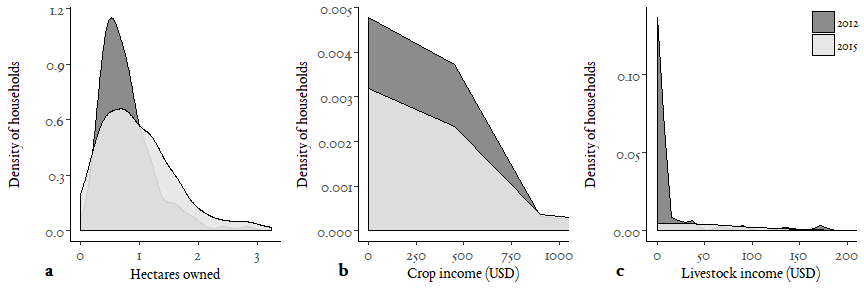
\includegraphics[width=1\textwidth]{figs_04/image2.png}
  \captionsetup{singlelinecheck = off, justification=justified}
    \caption{Distributions in 2012 and 2015 (a) Land owned (ha); b) Crop income (USD year$^{-1}$); c) Livestock income (USD year$^{-1}$)}
    \label{fig:04_1}
\end{figure}

Annual crop income was significantly lower in 2015; this was weakly related to changes in crop market orientation ($\hat{\alpha}$ = 64 (47), $\hat{\beta}$ = 394 (112) pr(\textgreater{\textbar}F{\textbar}) {\textless} 0.001, mixed-effects linear regression; Figure \ref{fig:04_2}), where some households decreased market participation and also decreased crop income, and others either remained stable or increased market participation and increased crop income.

There was no significant difference in vegetative index (EVI) between 2012, 2015 and the long-term annual average. Estimated rainfall, however, was more erratic in 2011 -- 2012, with approximately 90 mm more than average falling in November 2011 and approximately 90 mm less than average falling in May 2012. The most influential drought events (in terms of recorded crop yields), were recorded in both April 2011 (-100 mm) and April 2014 (-90mm), potentially influencing the main harvest recorded for each year (August 2011 and 2014; \citealp{Janowiak1999}). The effects of these rainfall differences are uncertain; harvests in 2012 may have been greater from the short rain planting period in 2011 (September -- November) and reduced for the long rain planting period in 2012 (February -- April).

\begin{figure}[H]
  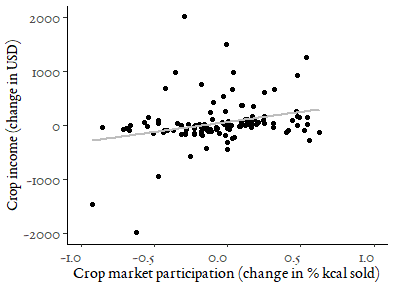
\includegraphics[width=0.6\textwidth]{figs_04/image3.png}
\captionsetup{singlelinecheck = off, justification=justified}
  \caption{Change in crop income (USD) and market participation (\% kcal sold), with regression line}
  \label{fig:04_2}
\end{figure}

The majority ({\textgreater}70\%) of households either did not have off-farm income opportunities or only earned a small proportion of their income from off-farm activities. In 2015, 3\% of households earned over 50\% of their income from off-farm activities, which is in contrast to 29\% of households in 2012. This change in off-farm income has no obvious explanation, but may indicate a lack of job security and a high risk of failure for off-farm businesses.

Observing these resources and farm characteristics over time, a diversity of concurrent changes are evident for a majority of households. Seventeen percent of households had a change in land area owned (${\pm}$ 1 ha). Seventy-seven percent of farmers show a change in land area owned, number of TLUs (${\pm}$ 2), market orientation of crops (${\pm}$ 50\%), market orientation of livestock (${\pm}$ 50\%), or changed crop diversity (${\pm}$ 2).

\subsection{Types of adaptive responses}

Four distinct groups were identified from the clustering process. Adaptive response clusters were named: `Rising high value crop' (n=25), `Rising livestock' (n=33), `Subsisting mixed' (n=42), and `Subsisting crops' (n=47; Table \ref{tab:04_2}).

Households in the `Rising high value crop' cluster were named based on their increased land area (64\% of households increased by {\textgreater} 0.25 ha), a larger allocation of land to non-staple crops (92\% of households), and their increased crop market participation. Increases in land area were allocated to tomatoes (29\% of households that increased land), potatoes (17\% of households) and coffee (16\% of households). Households in this cluster continued to cultivate staple crops, maintaining their high level of crop diversity over the three year period. Several households in this cluster also increased their livestock-holdings (predominantly cattle); the majority (73\%), however, reduced their market participation of livestock products. Twenty-four percent of households earned off-farm income in 2015, considerably less than the 56\% of households earning in 2012. Increases in land ownership indicate a shift in strategy for households in this cluster. While cultivating staple crops has been a consistent aspect of their farm strategy, cultivating high value crops may be a long-term strategy for some (e.g. 28\% of households had coffee bushes in 2012 and 2015), or a short-term tactic for others (e.g. 68\% of households added high value crops to their production mix in 2015).

Households in the `Rising livestock' cluster were named based on their increased land area (66\% increasing by {\textgreater} 0.25 ha), increased livestock-holdings (90\% of households) and their recent livestock market participation. These households also increased their cultivation and market participation of staple crops and cultivated a small portion of high value vegetables. Increases in land area were allocated to maize (60\% of households that increased land) and to a lesser extent increases in potatoes or tomatoes (14\%). Households that increased livestock-holdings generally did so by increasing cattle numbers (the majority of which were cross-bred or `exotic'), with a few exceptions of increased sheep and goat numbers. Livestock products were predominantly used for home consumption in both 2012 and 2015. Market participation of livestock products was not common in 2012; in 2015, however, 45\% of households in this cluster sold milk, eggs or home butchered meat. Live animals were marketed by the majority of households (51\%). Off-farm income was also earned by the majority of households (51\%) in 2015, ranging from 25 to 70\% of total income.

Households in the `Rising livestock' cluster sold live animals and increased livestock-holdings, indicating a viable long-term strategy, rather than short-term tactical destocking. The ownership of higher value mixed or `exotic' breeds (56\% of households) may also indicate a long-term strategy. Marketing of livestock products, however, may be a strategy for some (e.g. 15\% of households kept non-local cattle and marketed milk in 2015) and a tactic for others.

Households in the `Subsisting mixed' cluster, in general, maintained land-holdings, increased the portion of their land dedicated to staples and increased livestock-holdings. Crop and livestock market orientation decreased considerably when compared to 2012. The majority (65\%) of households kept cattle in 2012 and 2015, largely for home consumed milk production in 2015. Cattle keeping in the context of these communities is a considerable investment with barriers to procurement and sale; these households appear to be acting strategically on their asset ownership but may act tactically on whether to sell their milk or not.

Households in the `Subsisting crop' cluster reduced land cultivation, reduced crop market orientation and reduced livestock-holdings. The majority (91\%) kept poultry in both 2012 and 2015 indicating that livestock plays an important tactical role in this cluster; several households (29\%) ceased to keep cattle in 2015, indicating a potential strategic change.



\begin{sidewaystable}
  \captionsetup{singlelinecheck = false, justification=justified} %left justify caption
  \caption{
  Clustering variables by adaptive response cluster in 2012 and 2015 (median, IQR)
  }
  \label{tab:04_2}
  \small
%\begin{tabularx}{\textwidth}{@{}lYYYYYYYYYY@{}}
%  {
%p{\dimexpr 0.19\linewidth-2\tabcolsep}
%p{\dimexpr 0.09\linewidth-2\tabcolsep}
%p{\dimexpr 0.08\linewidth-2\tabcolsep}
%p{\dimexpr 0.07\linewidth-2\tabcolsep}
%p{\dimexpr 0.08\linewidth-2\tabcolsep}
%p{\dimexpr 0.08\linewidth-2\tabcolsep}
%p{\dimexpr 0.08\linewidth-2\tabcolsep}
%p{\dimexpr 0.08\linewidth-2\tabcolsep}
%p{\dimexpr 0.08\linewidth-2\tabcolsep}
%p{\dimexpr 0.09\linewidth-2\tabcolsep}
%p{\dimexpr 0.09\linewidth-2\tabcolsep}}
\begin{tabular}{L{3.8cm}cccccccc}
\toprule
 & \multicolumn{2}{C{3.6cm}}{\makecell{Rising high value crop \\ (n=25)}} & \multicolumn{2}{C{3.6cm}}{\makecell{Rising livestock \\ (n=33)}} & \multicolumn{2}{C{3.6cm}}{\makecell{Subsisting mixed \\ (n=42)}} & \multicolumn{2}{C{3.6cm}}{\makecell{Subsisting crop \\ (n=47)}} \\
 \cmidrule{2-9}
 & 2012 & 2015 & 2012 & 2015 & 2012 & 2015 & 2012 & 2015  \\
 \midrule
Household population (adult equivalents) & 3.84 (1.33) & 4.05 (2.3) & 3.81 (1.7) & 4.3 (1.8) & 3.88 (1.89) & 3.8 (1.44) & 3.3 (1.39) & 2.6 (1.62)  \\
Land owned (ha) & 0.71 (0.60) & 1.21 (0.81) & 0.71 (0.20) & 1.21 (0.81) & 0.71 (0.58) & 0.61 (0.81) & 0.61 (0.56) & 0.81 (0.81)  \\
Land cultivated (ha) & 0.71 (0.50) & 1.11 (0.81) & 0.71 (0.20) & 1.21 (0.81) & 0.71 (0.58) & 0.61 (0.49) & 0.61 (0.56) & 0.40 (0.41)  \\
Crop market participation$^{\mathrm{a}}$ & 30 (32) & 39 (23) & 23 (30) & 34 (38) & 29 (31) & 16 (30) & 19 (41) & 0 (25) \\
Crop diversity & 4 (3) & 4 (2) & 4 (3) & 4 (1) & 5 (2) & 3 (1) & 3 (3) & 2 (1)  \\
High value crops$^{\mathrm{b}}$ & 0 (9) & 22 (13) & 0 (10) & 0 (8) & 0 (4) & 0 (0) & 0 (0) & 0 (0)  \\
Livestock (TLUs) & 1.08 (1.85) & 1.9 (1.40) & 1 (1.39) & 2.91 (2.30) & 1.28 (1.24) & 1.82 (1.25) & 0.16 (1.40) & 0.05 (0.45) \\
Livestock market participation$^{\mathrm{a}}$ & 40 (75) & 0 (30) & 0 (0) & 0 (34) & 0 (73) & 0 (1) & 0 (0) & 0 (0) \\
Crop-livestock integration (\% practices) & 50 (50) & 100 (0) & 50 (50) & 100 (0) & 50 (0) & 100 (0) & 0 (50) & 50 (25) \\
Off-farm income (\% total) & 16 (52) & 0 (0) & 12 (73) & 25 (50) & 0 (26) & 0 (0) & 0 (46) & 0 (0)  \\
\bottomrule
\end{tabular}
\footnotesize
\raggedright
%\caption*{
\\
$^{a}$ Percent of calories produced.\\
$^{b}$ Percent of area cultivated. \\%}
\end{sidewaystable}




\subsection{Analysis of adaptive responses}

A range of non-clustering variables were considered as potential covariate attributes of the clusters. These included: gender of the household head, whether the household head changed, household structure (e.g. tri-generational, parent-child, individuals), aid (seed, fertiliser, food and financial), distance of plot (from homestead), fertiliser application, debt, elevation, SOC, soil acidity and average EVI in 2012 and 2015.

The gender of household head was significantly different between clusters ($\hat{\alpha}$ = -1.63 (0.30, $\hat{\beta}$ = 1.77 (0.44) pr(\textgreater{\textbar}{\chi}$^2${\textbar}) {\textless} 0.05, mixed-effects logistic regression, reference categories -- male head and non-`Subsisting crops'), with `Subsisting crops' having the highest instance of female-headed households (53\% of households), followed by `Subsisting mixed' (26\% of households). The gender and marital status of the household head can have land tenure implications, as well as implications on livestock ownership. In this case, there were significant differences in the full data set, with female heads cultivating less land than their male counterparts (pr(\textgreater{\textbar}F{\textbar}) {\textless} 0.001, Appendix Table \ref{tab:A_2}); and, female heads owning less livestock assets in 2015 (TLU; pr(\textgreater{\textbar}F{\textbar}) {\textless} 0.001, Appendix Table \ref{tab:A_2}). Within the `Subsisting' clusters, however, there were no differences between male and female heads in terms of land-holdings. In the `Subsisting mixed' cluster, male-headed households had significantly higher livestock-holdings (particularly cattle; pr(\textgreater{\textbar}F{\textbar}) {\textless} 0.05, Appendix A Table \ref{tab:A_3}).

Spatial analysis of a digital elevation model and soil property estimates (\citealp{Hengl2016}) of the study area showed that elevation was negatively correlated with pH and positively correlated SOC (r = -0.61, pr {\textless} 0.05; r = 0.79, pr {\textless} 0.01, Pearson's correlation). Despite this spatial variability, the modelled acidity and SOC levels would not present significant differences in crop or pasture constraints between clusters (e.g. pH was between 5.3 and 6.2 and optimal pH for maize in a nutrient solution is between 5.2 and 6.5; \citealp{Islam1980339}). It should be noted, however, that non-publicly available, finer scale modelling of the study area suggests that there is greater variability and instances of lower SOC than available at a 250 m resolution (compared to \citealp{Winowiecki2016263}).

Households in `Rising' clusters applied significantly more synthetic fertiliser per hectare in 2015 when compared to `Subsisting' households ($\hat{\alpha}$ = 3.85 (2.43), $\hat{\beta}$ = 8.98 (3.59) pr(\textgreater{\textbar}F{\textbar}) {\textless} 0.05, mixed-effects linear regression). Manure was often applied along with synthetic fertilisers, particularly for potatoes in `Rising' clusters and the `Subsisting mixed' households, as well as tomatoes and other vegetables in `Rising high value crops' households. Yields were significantly higher for households applying synthetic fertilisers to maize ($\hat{\alpha}$ = 719 (212), $\hat{\beta}$ = 813 (288) pr(\textgreater{\textbar}F{\textbar}) {\textless} 0.01, mixed-effects linear regression).

There was no statistically significant difference in receipt of aid, level of debt, distance of plot, household structure or EVI. Further, households in villages with ongoing interventions (potato and dairy) did not increase in scale or market orientation for those livelihood activities more than households in other villages.

\subsection{Outcomes of adaptive responses}

The distribution of crop incomes changed over time for all clusters, with median income increasing in `Rising' clusters and decreasing in `Subsisting' clusters (Figure \ref{fig:04_3}; $\hat{\alpha}$ = 7.57 (0.77), $\hat{\beta}$ = -4.30 (1.21) pr(\textgreater{\textbar}F{\textbar}) {\textless} 0.01, mixed-effects linear regression). The increased crop income in the `Rising high value crop' cluster was attributable to market vegetables such as tomatoes, rather than coffee which halved in price between 2012 and 2015.

\begin{figure}[H]
  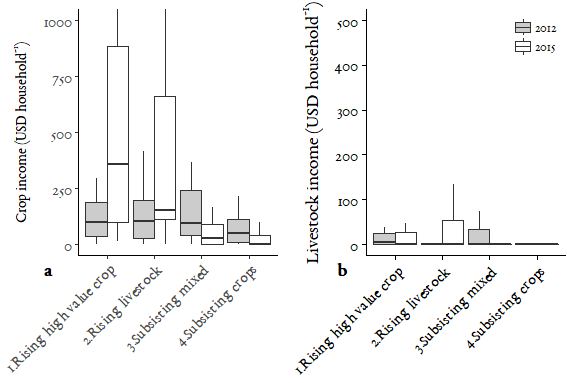
\includegraphics[width=0.6\textwidth]{figs_04/image4.png}
  \captionsetup{singlelinecheck = off, justification=justified}
    \caption{a) crop income (USD household$^{-1}$) by adaptive response cluster b) Livestock income performance (USD household$^{-1}$) by cluster}
    \label{fig:04_3}
\end{figure}
\vspace*{-3mm}

The distribution of livestock incomes did not differ significantly between 2012 and 2015. However, fresh milk producers in the `Rising' clusters generated significantly higher livestock incomes when compared to other households in the cluster ($\hat{\alpha}$ = 1.46 (0.36), $\hat{\beta}$ = 0.92 (0.40) pr(\textgreater{\textbar}F{\textbar}) {\textless} 0.01).

Households in the `Rising' clusters had significantly higher Food Availability scores and Household Diet Diversity Scores in the good period when compared to `Subsisting' clusters (Figure \ref{fig:04_4}; pr(\textgreater{\textbar}F{\textbar}) {\textless} 0.001, Appendix Table \ref{tab:A_4}).

In the lean period, `Subsisting crops' households had significantly less diverse diets than `Rising livestock' households ($\hat{\alpha}$ = 1.57 (0.07), $\hat{\beta}$ = 0.21 (0.10) pr(\textgreater{\textbar}{\chi}$^2${\textbar}) {\textless} 0.05, mixed-effects negative binomial regression). Households in the `Rising' clusters were significantly more food secure (in terms of access) than `Subsisting' households ($\hat{\alpha}$ = 9.48 (0.61), $\hat{\beta}$ = -2.28 (0.80) pr(\textgreater{\textbar}F{\textbar}) {\textless} 0.01, mixed-effects linear regression).

There was no significant difference in the PPI score; this is understandable as PPI is a slower moving indicator, requiring more time to see significant differences in performance.

Notably, there was no significant difference between clusters in the duration of the lean period (median = 3, IQR = 1), indicating that the pertinent issue is the intensity of hardship, rather than duration. Further, there was no significant difference in performance due to aid or gender of household head (results not shown).

\begin{figure}[H]
  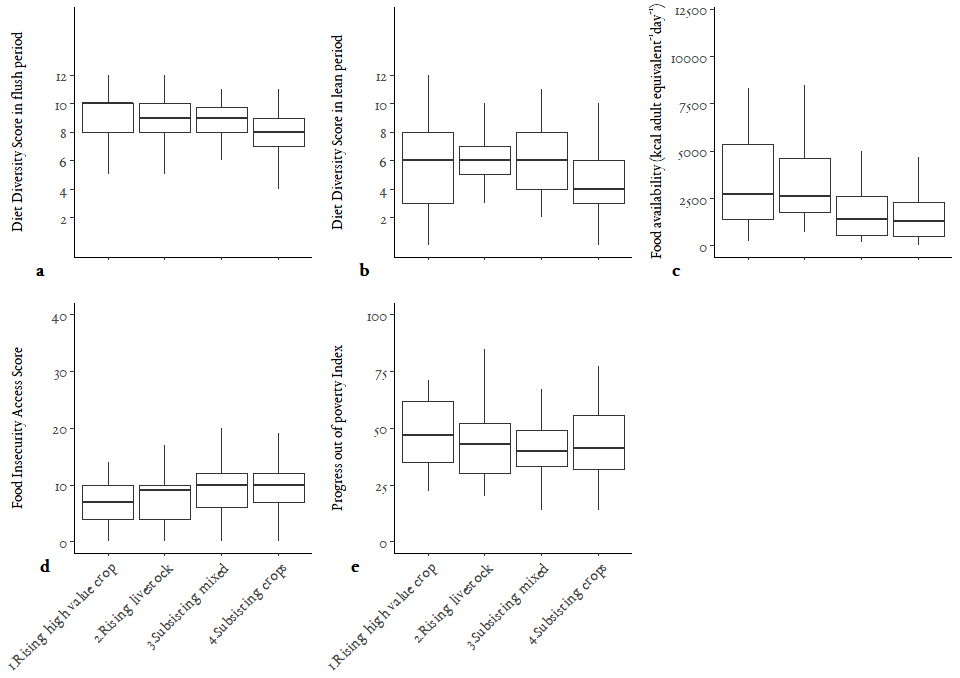
\includegraphics[width=1\textwidth]{figs_04/image5.png}
  \captionsetup{singlelinecheck = off, justification=justified}
    \caption{Performance indicators by adaptive response cluster in 2015. (a) Household diet diversity scores (HDDS) in the flush period; (b) Household diet diversity dcores in the lean period; (c) Food availability (kcal adult equivalent$^{-1}$ day$^{-1}$), including live animal sales; (d) Household food insecurity access scale (HFIAS); (e) Progress out of poverty index score}
    \label{fig:04_4}
  %\small
  %\raggedright

\end{figure}
\vspace*{-3mm}

\section{Discussion}

Households in the study site responded to local and national circumstances (e.g. drought months, regional and national economic growth) through a range of adaptive responses which have been classified as `Rising high value crop', `Rising livestock', `Subsisting mixed' and `Subsisting crops' (summarised in Table \ref{tab:04_3}). Overall, within the relatively short time period of three years (2012 -- 2015), 77\% of households made changes in farm resources or farm characteristics (Figure \ref{fig:04_1}a and Table \ref{tab:04_2}). Many of these changes can be classified as strategic, requiring considerable investment which will have an influence on the performance of the farming system over a longer period of time (e.g. 17\% of households changing land area by {\textgreater} 1 ha). Other observed changes (increases in vegetable production, changes in off-farm income) are more difficult to identify as long-term strategic changes as opposed to short-term tactics. A consequence of these rapid changes is that agency interventions need to be adaptable to maintain relevance for such farmers. Our results show that in sites like Lushoto with a good rural to urban connection (such as can be found in several regions of sub-Saharan Africa due to the many rapidly developing urban centres) projects are indeed aiming for a moving target and this will have implications on achieving income and food security outcomes, and requires targeted and rapid monitoring tools. There are valuable lessons that can be learned from this case study for macro development activities in the region (e.g. providing infrastructure and stimulating off-farm industries) as well as micro development activities (e.g. targeting and designing agency interventions).


%Alternative for this table https://latex.org/forum/viewtopic.php?t=8674
\begin{sidewaystable}
\captionsetup{singlelinecheck = false, justification=justified} %left justify caption
  \caption{
  Summary of changes in farm characteristics by cluster
  }
  \small
		%\centering
  \label{tab:04_3}
\begin{tabularx}{\textwidth}{
p{\dimexpr 0.18\linewidth-2\tabcolsep}
p{\dimexpr 0.08\linewidth-2\tabcolsep}
p{\dimexpr 0.08\linewidth-2\tabcolsep}
p{\dimexpr 0.08\linewidth-2\tabcolsep}
p{\dimexpr 0.08\linewidth-2\tabcolsep}
p{\dimexpr 0.08\linewidth-2\tabcolsep}
p{\dimexpr 0.08\linewidth-2\tabcolsep}
p{\dimexpr 0.08\linewidth-2\tabcolsep}
p{\dimexpr 0.08\linewidth-2\tabcolsep}
p{\dimexpr 0.08\linewidth-2\tabcolsep}
p{\dimexpr 0.08\linewidth-2\tabcolsep}}
\toprule
 & Land owned & Livestock holdings & Staple crops (\% area) & High value crops (\% area) & Crops marketed & Crops subsistence & Dairy marketed & Dairy subsistence & Poultry subsistence & Live animals marketed \\
 \midrule
Rising high value crops & ${\uparrow}$ H & ${\uparrow}$ M & ${\downarrow}$ M & ${\uparrow}$ H & ${\uparrow}$ H & {\textbullet} M & {\textbullet} L & {\textbullet} M & {\textbullet} H & M \\
Rising livestock & ${\uparrow}$ H & ${\uparrow}$ H & ${\uparrow}$ H & {\textbullet} L & ${\uparrow}$ H & {\textbullet} M & ${\uparrow}$ M & {\textbullet} M & {\textbullet} H & H \\
Subsisting mixed & {\textbullet} L & ${\uparrow}$ M & {\textbullet} H & {\textbullet} L & ${\downarrow}$ M & {\textbullet} H & {\textbullet} L & {\textbullet} M & {\textbullet} M & M \\
Subsisting crops & {\textbullet} L & ${\downarrow}$ L & {\textbullet} H & {\textbullet} L & ${\downarrow}$ L & {\textbullet} H & {\textbullet} 0 & ${\downarrow}$ L & {\textbullet} H & L \\
\bottomrule
\end{tabularx}
\footnotesize
\raggedright
%\caption*{
${\uparrow}$Increase in the cluster between 2012 and 2015 ${\downarrow}$ decrease in the cluster; {\textbullet} no significant change in the cluster. \\
L low level exhibited in cluster 2015; M medium; H high; 0 characteristic was not present in cluster.%}

\end{sidewaystable}



Some of the most substantial changes we observed in the three year period of study were most likely not related to any of the agency interventions that were being promoted in the region. Increases in land area, for example, coincided with increases in the tomatoes, potatoes, maize and coffee plantings. While there was active promotion of potato cultivation in Boheloi, there were no households in this village that increased land area and potato cultivation, suggesting that this intervention is not, in part, driving this land aggregation. The role that dairy interventions have had in increased livestock-holdings is also not clear. Dairy is actively promoted (through the `Maziwa zaidi' project branding -- bringing multiple partners and projects under the one banner) in four of the villages; households in the `Rising livestock' cluster that increased milk marketing, however, are spread out across the study site and so it is difficult to definitively attribute these changes to this intervention program.

The change of land expansion seen in the `Rising' clusters provides a counterpoint to the trend established in the literature of decreasing farm sizes across lower-income countries more broadly, and specifically in Africa (\citealp{HLPE2013}; \citealp{Jayne2003253}; \citealp{Lowder201616}; \citealp{Masters2013156}). On a national scale, \citet{Jayne2014} found that average farm sizes in Tanzania, being land abundant, had more than doubled between 1996 and 2003, with increases in land value making parents less willing to subdivide. The conditions for such expansion though, go beyond land value and also relates to the business viability of the farm. The business viability of land expansion depends on the potential to gain economies of scale (\citealp{Hazell20101349}), viable market opportunities and effective risk management (\citealp{Harris2014}).

Our clusters of change show some similarity to Dorward's classification of farm livelihoods (\citealp{Dorward2009}). Our `Rising' clusters can be compared to the `Stepping-up' group of households and `Subsisting' households can be equated to the `Hanging-in' group (\citealp{Falconnier2015}; \citealp{Valbuena20151395}), but this study shows these rural households can pursue completely different strategies. In general terms, Dorward's livelihood grouping can be a useful framework. In specific applications like in this study, however, it is not the most appropriate way of looking at farm household trajectories.

In an assessment of food availability of more than thirteen thousand households in sub-Saharan Africa, \citet{Frelat2016458} make predictions using variables related to livelihoods, namely: household size, number of livestock and land area. Notional food availability though, as seen in this study, does not necessarily translate to improvements in all aspects of food security. Specifically, significant differences in food availability between clusters are not present in HFIAS and HDDS in the lean period (Figure \ref{fig:04_4}), suggesting that it is necessary to include multiple metrics of food security, rather than food availability alone.

\subsection{Farm income and food security in Lushoto, Tanzania}

Regardless of adaptive response, farmers utilise resources with a high level of production risk and with no guarantee that crops or animal-sourced foods will be purchased above cost, if at all. Households in the `Rising high value crops' and `Rising livestock' clusters had a high degree of market orientation, with different approaches to market risk (Table \ref{tab:04_2}). The `Rising high value crop' households' decisions appear to have been financially beneficial, by cultivating more land, with a portfolio of coffee, tomatoes, market vegetables, staples as well as keeping livestock species. It may well be that the increased risk of their expansion strategy was mitigated by an astute set of tactics in response to crop market signals while maintaining or increasing a diversity of crop and livestock species (rather than specialising). The `Rising livestock' households' focus on livestock and staple crops also returned financial dividends; this is particularly the case for fresh milk producers in the `Rising' clusters, who are earning significantly more livestock revenue than other households and could indicate greater specialisation for these households (as theorised would happen in such favourable market conditions in \citealp{McIntire1992}). These clusters of households demonstrate how agile and fast moving households in the study area can be.

The higher performing `Rising' adaptive response clusters also present a challenge for external organisations seeking to replicate such performance. The complex risk management and market responsiveness that manifests as a diversity of crop and livestock products in these adaptive response clusters is at odds with single focus activities that external organisations tend to promote (as illustrated by free seed not translating into food security or diet diversity performance); further, the land expansion that this strategy depends on for its performance is risky. This potentially represents a future of winners and losers, ultimately with some landholders falling further into poverty rather than leveraging their agricultural enterprises to improve their well-being.

Longer term resilience of land-holding households is not guaranteed. Higher performance or subsistence at the expense of the natural resource base can only be sustained for so long. Ongoing cultivation with minimal fallow and low inputs will work to deteriorate soil health in the future, limiting crop and pasture production. Households keeping ruminant livestock species (`Rising' and `Subsisting mixed') managed integrated crop-livestock systems, which is a positive attribute in terms of yields and soil health.

\section{Conclusions}

This study observes livelihood dynamics and related poverty and food security performance over a three year period in a high potential, market connected region of Tanzania. Evidence suggests that 1) the drivers for the most significant livelihood changes do not necessarily relate to agency interventions; 2) the adaptive responses that have been implemented in this community incorporate multiple components (e.g. off-farm income, diverse crops and livestock) and are relatively heterogeneous across the study site; and 3) there is a partial disconnect between potential food availability (from income and kcal production) and short and long-term food security. Such evidence has implications for development agendas.

A substantial portion of households in the study site made changes to their livelihoods over the short three-year period analysed in this paper. Changes in land ownership, livestock-holdings and high value crop production are most likely related to market opportunities and personal circumstances, rather than direct interventions. Several households are making substantial strategic changes by expanding land ownership, planting perennial crops and investing in exotic cattle breeds; many households are also tactically utilising their land for diversified, mixed crop-livestock production. The majority of households, however, have either remained stable or are scaling back to subsistence farming. Households that are expanding their land area, present a unique case study in sub-Saharan Africa, where households in land scarce regions (albeit in a land abundant country) are consolidating land, with the potential to gain economies of scale.

Government and non-government organisations face challenges in designing interventions that remain relevant to such rapidly changing rural households, with multifaceted livelihoods and varying `well-being priorities'. This study highlights, the need for interventions to simultaneously support a diversity of livelihood activities (e.g. dairy, staples and post-farm value chain) targeted at clusters of households. Monitoring of income and food availability is not sufficient to measure well-being, rather multiple well-being indicators are needed.

\section{Acknowledgements}

We thank all the people involved in the conversations that formed the basis for this study and especially the farmers for sharing their valuable time. We also thank the three anonymous reviewers for their comments and insights. This work is a joint output of the CGIAR Research Programs on `Livestock and Fish', `Climate Change, Agriculture and Food Security' (CCAFS) and `Maize'. The work was also supported by the USAID-funded Feed the Future Sustainable Intensification Innovation Laboratory. The views expressed in this paper can not be taken to reflect the official opinions of these organisations.
